\documentclass[12pt,a4paper]{amsart}

\usepackage[utf8]{inputenc}
\usepackage{amsmath}
\usepackage{amsfonts}
\usepackage{amssymb}

\usepackage{hyperref}

\usepackage{float}
\usepackage{subfig}


%\usepackage[dvipdfmx]{graphicx}
\usepackage{graphicx}
\usepackage{caption}
%\usepackage[nobysame, alphabetic]{amsrefs}
%\usepackage{here}
%\usepackage{showkeys}
\newcommand{\modif}{$\clubsuit$}
\newtheorem{thm}{Theorem}[section]
\newtheorem{defn}[thm]{Definition}
\newtheorem{coro}[thm]{Corollary}
\newtheorem{prop}[thm]{Proposition}
\newtheorem{lem}[thm]{Lemma}
%\theoremstyle{definition}
\newtheorem{rmk}[thm]{Remark}
\newtheorem{cond}[thm]{Condition}

%CB defs
\def\HH{\mathbb{H}}
\def\dHH{\partial \mathbb{H}}
\def\HHn{\HH^n}
\def\hd{\hat{\delta}}
\def\ha{\hat{\alpha}}
\def\haa{\ha \cup \{\alpha^+,\alpha^-\}}

\def\im{\mathrm{Im}\,}



\def\SL{\mathrm{SL}(2,\CC)}

\def\xx{\HH/\Gamma'}


\def\ZZ{\mathbb{Z}}
\def\CC{\mathbb{C}}
\def\RR{\mathbb{R}}
\def\QQ{\mathbb{Q}}
\def\NN{\mathbb{N}}

\def\tt{\Sigma_{1,1}}

\def\fp{\mathbb{F}_p}
\def\aut{\text{Aut}(\F2)}
\def\gl2{\mathrm{GL}(2, \ZZ)}
\def\sl2{\mathrm{SL}(2, \ZZ)}
\def\g2{\Gamma(2)}
\def\GG{G_m}
\def\slc{\mathrm{SL}(2, \CC)}

% \def\xx{\HH/\g2}
\def\gg{\mathcal{G}_n}
\def\ggp{\mathcal{G}_p}

\def\isom{\mathrm{isom}(\HH)}

\def\isomH{\text{isom}^+(\HH)}
\def\tr{\text{tr\,}}


\def\GI{\mathbb{Z}[i]}
\def\hc{\CC \setminus \GI}



\title{Markov uniqueness, pants and the Bunyakovsky conjecture}

 \author[McShane]{Greg McShane}
 % \author[Vlad]{Vlad Sergesciu}
\address{Institut Fourier 100 rue des maths, BP 74, 38402 St Martin d'H\`eres cedex, France}
\email{mcshane at univ-grenoble-alpes.fr}


\begin{document}

\maketitle

\begin{abstract} 

We show that the Bunyakovsky conjecture implies the Markov uniqueness
conjecture. Explicitly: If for every positive integer $m$ the sequence 

$$k^2m^2 + 1, k \in \ZZ$$ 

contains a prime then Markov uniqueness conjecture is true. Surprisingly,
though our result relates these two well known conjectures in number theory, 
the ingredients of   our proof are for the most part geometric and to some extent
topological.

\end{abstract} 


\section{Introduction}

\subsection{Markoff numbers}

A \textit{Markoff triple} is a  solution $(X,Y,Z)$  in positive integers to
the \textit{Markoff cubic}
\begin{equation}\label{m cubic}
X^2 + Y^2 + Z^2 - 3XYZ = 0.
\end{equation}

A Markoff triple is said to be \textit{normalised} iff $z> y > x$, Aside from
the two smallest singular triples $(1,1,1)$ and $(1,1,2)$, every Markov triple
consists of three distinct integers. A \textit{Markoff number} is an integer in
a Markoff triple.

\subsection{Uniqueness of Markoff Numbers}
 
The unicity conjecture, apparently a question asked by Frobenius, says that the
largest number in a Markoff triple determines the remaining two numbers or
alternatively that any Markoff number greater than 2 belongs to a unique
normalised triple. Button and Baragar (see chapter 10 of Aigner \cite{aigner})
used  basic algebraic number theory to show that certain Markoff numbers
satisfied the uniqueness conjecture.  

 \begin{thm}[Baragar, Button, Schmutz] \label{button}
 Let $m$ be a Markoff number of the form 
 $m=p^k$ or $m=2p^k$ then it is unique
if $p$ is an odd prime.
 \end{thm}


Subsequently Aigner extended  this approach showing:
 
 \begin{thm}[Aigner]
 Let $m$ be a Markoff number of the form 
 $$m =Np^k$$
 where $p$ is an odd prime and $N \leq 10^{35}$ is another Markoff number. Then $m$ is unique.
 \end{thm}

We will not be concerned with Aigner's theorem but we will give a short proof
of Button's theorem using some geometry and the fact that the ring of Gaussian
integers is a unique factorisation domain. This geometric approach will allow
us to show that the unicity of Markoff numbers is a corollary of the
Bunyakovsky conjecture. More precisely:

\begin{thm}\label{main}

If for every positive integer $m$ the sequence $$k^2m^2 + 1, k \in \ZZ$$ contains a
prime then the uniqueness conjecture is true.

\end{thm}

The polynomial $m^2 X^2 + 1$ satisfies the hypothesis of the Bunyakovsky conjecture:
\begin{itemize}
\item its leading coefficient is positive.
\item it is irreducible over $\ZZ$.
\item it is non trivial over $\mathbb{F}_p$ for all primes $p$.
\end{itemize}

According to the conjecture under these hypotheses the the restriction of the
polynomial  $m^2 X^2 + 1$ to the integers has an infinity of prime values.

The proof of our theorem, though it relates two conjectures apparently from
number theory, has an essential topological ingredient in the form of Lemma
\ref{lem: labelling}.


\subsection{Geodesics on hyperbolic surfaces} In the mid 20th century H. Cohn
initiated a program which resulted in a correspondence between Markoff numbers
and the lengths of simple closed geodesics on the modular torus. Recall that
the \textit{modular torus} is the surface obtained as the quotient of the
Poincar\'e half space $\HH/\Gamma'$ where $\Gamma' < P\sl2$ is the commutator
subgroup. The correspondence can be stated as follows, if $\gamma$ is such a
geodesic then: 

\begin{equation} X  = \frac{2}{3} \cosh \left(
\frac{\ell_\gamma}{2}\right),
\end{equation} 

is a Markoff number where
$\ell_\gamma$ is the length of $\gamma$. Conversely, every Markoff number
arises as the length of such a geodesic.

There is an equivalent conjecture to the Markoff conjecture (Conjecture 3
\cite{mcp}) which concerns simple closed geodesics on $\xx$:

\textit{The modular torus $\xx$ has the following property: if $\alpha, \beta$
is a pair of simple closed geodesics of the same length, then there is an
automorphism  of $\xx$ taking one to the other.}

Since the group of automorphisms of $\xx$ is isomorphic to a cyclic group of order 6 
this means that the multiplicity of and number in the spectrum of  lengths is at most 6.

\begin{figure}[ht]
\begin{center}
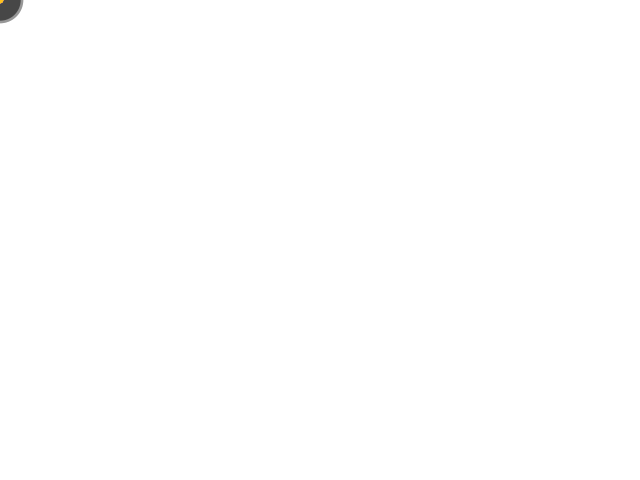
\includegraphics[scale=.5]{torus.png} 
\end{center}
\caption{A punctured torus with a closed simple geodesic $\alpha$ and the arc $\alpha^*$ disjoint from it. The shaded area is a cusp region.}
	\label{fig:torus}
\end{figure}

An important feature of the $\xx$ is that it admits non trivial automorphisms.
It is east to show that $\Gamma'$ is normalised by $\begin{pmatrix} 0 & -1 \\ 1 & 0
\end{pmatrix}$ and so this induces an automorphism, in fact the
\textit{elliptic involution}, of $\xx$. A  \textit{Weierstrass point} is one of
the three fixed points of this involution. The interaction of this
automorphisms with the various geodesics on $\xx$ is central to the proof of
Theorem \ref{main}.

\subsection{Introducing $\lambda$-lengths}

% We discuss the connection between $\lambda$-lengths and Markoff numbers proving
% that every such number is the sum of two squares in a natural geometric manner.

The closed geodesics form an interesting class of curves that has been much
studied not just in relation to the Markoff numbers. There is another class of
curves, namely the \textit{bicuspidal geodesics or arcs}, that have also proved
to be important in many contexts for example Penner's theory of moduli space of
surfaces with marked points and more recently cluster algebras. Though each arc
is non compact and so has infinite length Penner \cite{bob} introduced a
modified notion of length, \textit{$\lambda$-length}, which allows one to
perform useful calculations.  Penner's $\lambda$-length of simple bicuspidal
geodesic on a punctured surface is essentially the exponential of  the length
of the portion outside of some fixed system of cusp regions. Recall that a
\textit{cusp region} in a hyperbolic surface is a portion of the surface
isometric to  the quotient of $\{ z, \im z > 1\}$ by the action of the group
generated by $z \mapsto z + A, A > 0$. A simple calculation shows that the area
of the cusp region is $A$ (see \cite{thesis} for a discussion). On the modular
torus there are two natural choices for the cusp region :

\begin{itemize}
\item the universal cusp region $H_2$  of area $2$ present on any cusped hyperbolic surface.
\item the  maximal cusp region $H_6$ of area $6$ 
\end{itemize}
(see \cite{thesis} for details).

For the purposes of this paper we will uses a slightly more general notion of
$\lambda$ length: Let $\gamma$ be a bicuspidal geodesic and $H$ be a cusp
region and choose a lift of  
$\gamma$, $\hat{\gamma}\subset \HH$,
joining $\gamma^\pm \in \partial \HH$.
The \textit{$\lambda$-length} of $\gamma$ with respect to $H$ is
defined to be the exponential of the length of the portion of $\hat{\gamma}$ 
outside of the pair of lifts of $H$ tangent to $\partial \HH$ at $\gamma^\pm$.

\begin{figure}[ht]
\begin{center}
\includegraphics[scale=.5]{lambda.png}
\end{center}
\caption{Lift of $\gamma$ and the terminal lifts of the cusp region $H$.
The solid arc of the demi circle is the portion used to define the $\lambda$-length  with respect to $H$.}
	\label{fig:lambda length}
\end{figure}

 By using calculations in Wolpert \cite{saw} we will see that, for the maximal
 cusp region on the modular torus,  the $\lambda$-lengths of arcs coincide with
 the squares of Markoff numbers. More precisely:
 
\begin{thm}\label{thm:triangulation lengths}
For each  Markoff triple $(X,Y,Z)$
there is a (unique) ideal triangulation of the modular torus
such that the $\lambda$-lengths of the arcs are 
$X^2,Y^2,Z^2$.
\end{thm}

 Then, using the fact that each arc is invariant under the elliptic involution
 one can show, by applying Lemma \ref{squares}, that every Markoff number is
 the sum of two squares that is it factorises over the Gaussian integers.

 \subsection{Idea of the proof}

Our proof of Button's theorem is based on the following ingredients: 
\begin{itemize}
\item each closed simple geodesic $\alpha$ on $\xx$ is paired with a unique arc (simple bicuspidal geodesic) $\alpha^*$. 
\item each arc passes through a single Weierstrass point on the punctured torus
\item a reformulation (Theorem \ref{frobenius}) of the unicity conjecture in terms of multiplicities for lengths of simple geodesics (see \cite{mcp}).
\end{itemize}


On closer examination one sees that we don't actually need the bicuspidal
geodesic to be simple only that it be both disjoint from $\alpha$,
is invariant under the elliptic involution, 
and have $\lambda$-length a prime which does not need to be a Markoff number. 

\subsubsection{Key topological lemma}
It is important to note here that any pair of
distinct simple closed geodesics on the punctured torus is \textit{filling}
that is the complement consists of a union of discs and a punctured disc. It
follows from this that:

\begin{lem}\label{lem: labelling}
On a punctured torus any bicuspidal geodesic, whether simple or not, is
disjoint from at most one closed simple geodesic.
\end{lem}

\begin{figure}[ht]
\begin{center}
\includegraphics[scale=.5]{cut_torus.png}
\end{center}

\caption{Above a pair of simple closed geodesics $\alpha$ and $\beta$ on the
punctured torus. When we cut along the geodesics we obtain the punctured disc
below.}

	\label{fig: cut torus}
\end{figure}

\subsubsection{Proving unicity for a Markoff number} Our argument now is that
if $\gamma, \gamma'$ is a pair of  bicuspidal geodesic 

\begin{itemize}	
\item each of which is invariant under the elliptic involution 
\item have $\lambda$-length a prime $p$ 
\end{itemize}	

then there is an automorphism of $\xx$ which takes $\gamma$ to $\gamma'$. This
is because  the prime $p$ splits in an essentially unique way over the Gaussian integers.
This means that there are at most six such geodesics on $\xx$. Now if $\gamma$
is in addition disjoint from a simple closed geodesic $\alpha$ then any other
simple geodesic of the same length is the image of $\alpha$ under some
automorphism of $\xx$ too. (see discussion of Conjecture 3 \cite{mcp} above).

% \begin{thm}[Fermat]\label{main}
% Let $p$ be a prime then the equation
% $$x^2 + y^2 = p $$
% has a solution in integers  iff  $p =2$ or $p-1$ is a multiple of $4$.
% \end{thm}

% As in Zagier's remarkable proof \cite{zagier} this result follow from showing
% that a certain involution has a fixed point. Amusingly Burnsides's Lemma
% reduces this to showing that another involution has exactly two fixed points.


\subsection{Organisation, Remarks}

In Section 2 we recall the definition of Ford circles and discuss their
relation to the geodesics of the Poincaré half plane. We study the orbit of the
imaginary point $i$ under $P\sl2(\ZZ)$ and how this relates to the
representation of an integer as the sum of two squares. Section 3  is an
exposition of the Markoff cubic viewed as the character variety of the free
group on two generators. We then explain how to pass to $\lambda$-lengths and
prove Theorem \ref{thm:triangulation lengths}. In Section 4 we prove Button's
theorem using the results of Sections 2 and  3.  Finally we extend this proof
to show Theorem \ref{main} and show how the sequence $k^2m^2 + 1$ arises. 


The content of sections 2 and 3 is purely expository and, as such, we make no
claims of originality. We will assume that the reader has some familiarity with
the theory of Fuchsian groups. Almost all  of the material in Sections 2 be
found in Serre's book \cite{serre} and the reader should not need any other
references to understand this paper. 

This work grew out of an attempt to find a geometric proof of Fermat's theorem
on sums of squares to understand Heath-Brown and Zagier's proofs \cite{zagier}.
We note that in recent work by Bourgain, Gamburd and Sarnak prove that almost
all Markoff numbers are highly composite. Much inspiration came from listening
to Dennis Sullivan's lecture at the Abel Prize ceremony in 2022. The idea of
looking at other arcs on pants is how I fancifully imagined he, as a
topologist, might have tried to deal with composite Markoff numbers.

 % \subsubsection{Farey tessalation}
% This work was  inspired by an almost obsessive study  of the 
 % \textit{Farey tessalation}.
 

\subsection{Thanks}

The first author thanks Bob Penner, Louis Funar and Alexei Marin
conversations over the years concerning this subject. He would also like to
thank Xu Binbin for reading early drafts of the manuscript.

We would also like to thank Boris Springborn  for telling us about his work
\cite{spring} which is closely related to ours.

\hfill $\Box$


\section{Ford circles, lengths, midpoints} 
\label{lengths}

We denote by $F$ the set  $\{ z, \im z > 1\}$ this is a \textit{horoball in
$\HH$} centered at $\infty$. The image of $F$ under the $\sl2$ action consists
of $F$ and infinitely many disjoint circles, the so-called \textit{Ford
circles}, each tangent to the real line at some rational $m/n$. We adopt the
convention that $F$ is also a Ford circle of infinite radius. Our interest in
Ford circles stems from:

\begin{lem}
The Ford circles are invariant under $\Gamma'$ and their projection to $\xx$ 
is the maximal cusp region $H_6$ of area $6$.
\end{lem}

\proof The Ford circles are invariant under $\Gamma'$ and so project to a cusp
region on $\xx$. The stabiliser of $F$ in $\Gamma'$ is the group generated by
$z \mapsto z + 6$. Now the area of the cusp region is $6$ by the formula for
the area of a cusp region. \hfill $\Box$

\begin{figure}[ht]
\begin{center}
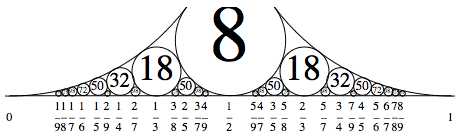
\includegraphics[scale=.8]{Ford-circles.png} 
\end{center}
\caption{Ford circles with tangent points and curvatures.
Recall that the curvature of a euclidean circle is twice  the square of  the reciprocal of its radius.}
\end{figure}

The following is well known and is easily checked:

\begin{lem}\label{ford}
The Ford circle tangent to the real line at $m/n$
has Euclidean diameter $1/n^2$.
\end{lem}


We define the \textit{length} of the vertical line 
$\{ k/p + i t,\, t \in \RR \}$
to be the length of the  sub arc joining 
$F$ to the Ford circle tangent at $k/p$.
Further we define its  \textit{mid point} to be the midpoint of this sub arc.
We remark that if the projection of the line to $\xx$
is invariant by an automorphism 
then the midpoint is necessarily a fixed point of the automorphism.

The following is a restatement of Lemma \ref{ford} in terms of these notions:

\begin{lem}.\label{calcul}
Let $m/n$ be a rational. 
Then the geodesic $\{ m/n + i t,\, t \in \RR \}$
\begin{itemize}
\item has  length $2\log n$. 
\item has its midpoint at $ \frac{1 }{n}(m + i).$
\end{itemize}
\end{lem}

Finally, the key lemma that relates the $\sl2$ action to sums of squares is:

\begin{lem} \label{squares}
Let $n$ be a positive integer.
The number of  ways of writing $n$  as a  sum of squares
$$n = c^2 + d^2$$
with $c,d$ coprime integers
is equal to the number the  integers $0 \leq k < n-1$ coprime to $n$
such that the line
$$\{  k/n + i t,\, t \in \RR \}$$
contains  a point in the $\sl2$  orbit of $i$.
\end{lem}


\proof  Suppose there is such  a point which we denote  $w$.
The point $w$ is a fixed point of some  element of order 2 in $\sl2$.
Since the Ford circles are $\sl2$ invariant
this element must permute $F$ with the Ford circle tangent 
to the real line  at the real part of $w$.
So, in particular, $w$ is the midpoint of the line 
that it lies on 
and by  Lemma \ref{calcul} one has:

$$\frac{1}{n} = \im \frac{1 }{n}(k + i)  
= \im  \frac{ai +b}{ci+d }
= \frac{\im i} {c^2 + d^2}.$$

Conversely if $c,d$ are coprime integers 
 then there exists $a,b$ such that
 $$ad - bc = 1 \Rightarrow  
 \begin{pmatrix}
 a & b \\
 c & d
 \end{pmatrix} \in \sl2.
$$
%The real part of $w = \frac{ai +b}{ci+d }$ is
%$$ac + bd = (a,b).(c,d),$$
%and
By applying a suitable power of the parabolic transformation 
$z \mapsto z + 1$,
one can choose $w$ such that $0 \leq \text{Re\,} w < 1$.
So if $n = c^2 + d^2$ then $\frac{ai +b}{ci+d }$
is on one of the lines of the family in the statement.

\hfill $\Box$

\subsubsection{Calculating $\lambda$-lengths}

Let $a/c, b/d$ be a pair of distinct rationals. We define the \textit{length}
of the arc joining these rationals to be the length, with respect to the
Poincar\'e metric on $\HH$, of the portion  outside of the Ford circles tangent
at $a/c, b/d$ . and the $\lambda$-length of an arc to be the exponential of
this length. It is a consequence  of Lemma \ref{calcul} below  that the arcs of
$\lambda$-length 1 are the edges in the so-called \textit{Farey diagram} (see
Figure \ref{farey diagram}). We have:

\begin{lem}\label{calcul}
Let $a/c, b/d$ be a pair of distinct extended rationals.
Then the  $\lambda$-length of the arc joining them
 is the square of the determinant of the matrix
$$\begin{pmatrix}
a & b \\ c & d
\end{pmatrix}.$$

Further if $a/b = 1/0$ then the arc is a vertical line 
 whose midpoint has imaginary part equal to $1/d$ .
\end{lem}

\proof 
By transivity of $P\sl2$ on the extended rationals we may assume 
$a/c = 1/0$ and so the determinant of the matrix is $d$.
The Ford circle at $1/0$  is $\{ z, \im z > 1\}$ and
at $b/d$ it is a circle of euclidean diameter $1/d^2$.
The top of this circle is tangent to the line $\{ z, \im z = 1/d^2\}$
and the $z \mapsto d^2 z $ maps this to the boundary 
of the Ford circle $\{ z, \im z \geq 1\}$.
It is easy to see that the distance between these sets,
and so the length of the segment outside the Ford circles,
is $2\log d$. Thus the $\lambda$-length is the square of the 
determinant as required.

\hfill $\Box$


 
\section{Markoff cubic and the character variety}

In this section we give a short modern exposition of the basis of H. Cohn's
approach.

\subsection{Character Variety}

It is convenient to change variables and study solutions of
\begin{equation}\label{f cubic}
X^2 + Y^2 + Z^2 - XYZ = 0.
\end{equation}
By the work of Fricke the set of solutions in positive real numbers
can be identified with a certain slice of the 
\textit{relative character variety of $\ZZ * \ZZ$}.
This is the set of  representations 
$$\rho: \ZZ * \ZZ \rightarrow SL(2, \RR)$$
such that the trace of the image of the commutator of the generators is $-2$
up to conjugation.
The key point in Fricke's work is that an (irreducible) representation $\rho$
is determined up to conjugation by the three numbers
\begin{eqnarray*}
X &= &tr \rho(\alpha), \\
Y  &= &tr \rho(\beta), \\
Z &= & tr \rho(\alpha\beta)),
\end{eqnarray*}
where $\alpha,\beta$ are generators of $\ZZ*\ZZ$.
Fricke calculates the trace of the commutator and shows that
\begin{equation}
2 + tr\,  (\alpha\beta\alpha^{-1}\beta^{-1}) = X^2 + Y^2 + Z^2 - XYZ .
\end{equation}
The quotient surface $\HH/\rho(\ZZ*\ZZ)$ is invariably a once punctured torus
and we identify $\ZZ * \ZZ$ with its fundamental group.
The $\alpha\beta\alpha^{-1}\beta^{-1}$ is a loop around the puncture
and the condition of the trace means that the monodromy around this loop is parabolic.


\subsection{More $\lambda$ lengths}

There is an embedded cusp region $H_4$  of area $4$ on any punctured torus
$\HH/\rho(\ZZ*\ZZ)$ and on the modular torus $\xx$ there is a maximal cusp
region $H_6$ of area $6$ (see \cite{thesis} for a discussion).
% We choose a represention $\rho$ such that its image is $\Gamma'$.
After possibly replacing $\rho$ by a conjugate representation we may assume
$\rho(\ZZ*\ZZ)$  that $$\rho(\alpha\beta\alpha^{-1}\beta^{-1}): z \mapsto z +
6,$$ it follows that $H_4$ lifts to the set $\hat{H} = \{ \im z > 3/2 \}$. Let
$\alpha*$ be an\textit{arc} that is a bicuspidal geodesic without self
intersetions. There is a lift of $\alpha*$ to $\HH$ which is a vertical line
which evidently meets $\hat{H}$, we claim that any lift of of $\alpha*$ which
meets $\hat{H}$ is a vertical line and not a semi circle. For, if $C$ is a semi
circle that meets $\hat{H}$ its diameter is strictly greater than $6$ and it
follows that $C$ and $C + 6$ meet transversely in some point $x$. Such a point
gives rise to a self intersection on the quotient surface It follows that, the
portion of $\alpha^*$ outside of $H$ is connected, and we define
$\lambda$-length  of $\alpha^*$ to be the exponential of the length of this sub
arc.

\begin{lem}\label{lambda length}
Let $\alpha*$ be an arc on a once punctured torus 
and $\alpha$ the unique 
simple closed geodesic disjoint it.
Then the square root of the $\lambda$-length  of the arc $\alpha$
is equal to $\frac{2}{3}\cosh \ell_\alpha / 2$.
\end{lem}

It is possible to prove this directly using hyperbolic trigonometry 
following the same schema as in \cite{thesis}
but here we give a more conceptual proof  using the computations from \cite{saw}
the interested reader should also consult \cite{yi thesis}.

Given an arc $\alpha^*$ one may extend it to an ideal triangulation of the
punctured torus: that is there is a pair of arcs $\beta^*,\gamma^*$, each
disjoint from  $\alpha^*$ and the complement of $\alpha^* \cup \beta^* \cup
\gamma^*$ a pair of ideal triangles. Let $X$ denote $2 \cosh \ell_\alpha / 2$
where $\alpha$ is the unique closed simple geodesic disjoint from $\alpha$ and
likewise

\begin{equation*}
Y = 2 \cosh \ell_\beta / 2 ,\,\, Z  = 2 \cosh \ell_\gamma / 2 
\end{equation*}
where $\beta$ resp $\gamma$ is the unique closed simple  geodesic disjoint from
$\beta^*$ resp. $\gamma^*$.

\begin{figure}[ht]
\begin{center}
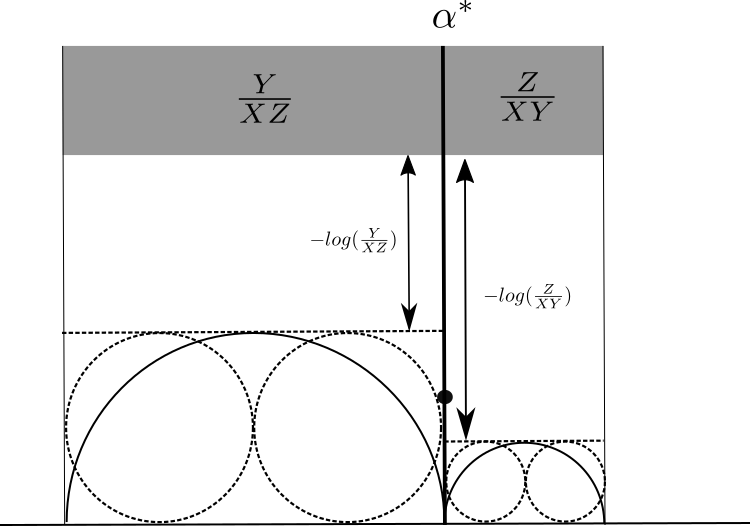
\includegraphics[scale=.5]{shear.png} 
\end{center}
\caption{Calculating the hyperbolic length of $\alpha^*$ in the upper half plane
the $\lambda$-length is the exponential of this.
The mid point of $\alpha^*$ is marked by a circle and
the two corners adjacent to $\alpha^*$ are shaded}
\label{penner}
\end{figure}

In  \cite{saw} Wolpert divides the Markoff cubic by $XYZ$ to obtain
$$\frac{X}{YZ} + \frac{Y}{XZ} + \frac{Y}{XZ} = 1.$$
The three terms in this relation have a geometric interpretation
which we will exploit to compute the $\lambda$-length of $\alpha^*$.
Let $H$ denote the cusp region of area $2$. 
A\textit{corner} of an ideal triangle is one of the 
three components of its intersection with $H$.
Every torus admits an \textit{elliptic involution}
which leaves each of the arcs of the ideal triangulation  invariant
 and swaps the triangles.
So, in fact, to each triangulation we can associate three numbers
namely the areas of the corners of one of the  ideal triangles
and these coincide with Wolpert's three numbers.

Lifting the ideal triangulation to $\HH$ as in Figure \ref{penner}
one sees that  $\alpha^*$ decomposes into two arcs of length
$-\log(Y/XZ)$ and $-\log(Z/XY)$ respectively
so that its is of length $2\log X$.

So, on any hyperbolic punctured torus,
the $\lambda$-length of $\alpha^*$ wrt the cusp region of area 2 is
the exponential of this, that is:
$$ X^2.$$
Now on the modulaire torus $\HH/\Gamma'$ there is an embedded cusp 
region of area 6 and the $\lambda$-length of $\alpha^*$ wrt this cusp region
is
$$ \frac{X^2}{9}.$$



\subsection{Sum of squares}\label{frobenius}


In the proof of Lemma \ref{lambda length} we used the fact that every torus
admits an \textit{elliptic involution} which leaves each of the arcs of the
ideal triangulation  invariant and swaps the triangles. For the modular torus
the involution is covered by $z \mapsto -1/z$ and  this means that for any arc
$\alpha^*$ every lift contains a point of the $\sl2$-orbit of $i$. In
particular, by Lemma \ref{lambda length}, a lift which is a vertical line ends
at a rational which has as denominator a Markoff number and so this Markoff
number is a sum of two squares. Conversely, every Markoff number arises as the
square of a $\lambda$-length of some arc  $\alpha^*$ and so must be the sum of
two squares. By extending this reasoning slightly (compare \cite{mcp} and
\cite{spring}) we obtain:
 
 \begin{thm}
The uniqueness conjecture is equivalent to: \newline
Let $m$ be a Markoff number then exactly one of the vertical lines
with endpoint  $k/m$, where $1\leq k \leq m-1$ is coprime to $m$,
projects to an arc on the modular torus.
\end{thm}

\proof The Markoff triples form a binary tree with a preferred vertex
corresponding to the fundamental triple $(1,1,1)$. Define the multiplicity of a
Markoff number to be the  number of triples for which it appears as the largest
integer. One can easily check that for the so-called singular Markoff numbers 1
and 2 their multiplicity is 3 and, since group of automorphisms of the tree
that fix the fundamental triple of order 6, the multiplicity of any other
Markoff number is at least $6$. Thus the uniqueness conjecture can be restated as:
multiplicity of any other Markoff number is at most $6$.

Using Cohn's correspondence it follows that the uniqueness conjecture is equivalent
to the number of oriented closed simple geodesics on the modular torus of any
given length is at most 6. Each (unoriented) closed simple geodesic is disjoint
from exactly one arc so that there can be at most three arcs of any given
$\lambda$-length.

The group of orientation preserving  automorphisms of the modular torus 
is canonically isomorphic to 
$$\sl2 / \Gamma' \simeq \ZZ/3\ZZ \times \ZZ/2\ ZZ \simeq \ZZ/6\ZZ .$$
The commutator of the generators of $ \Gamma'$  is $z \mapsto z + 6$
and since each automorphism $\phi$ must leave the cusp invariant it lifts to
a map of the form $\hat{\phi} : z \mapsto z + k,\, k= 0,\dots 5$.
Now consider the lift of some arc on the modular torus 
which, WLOG, is a vertical line. 
After applying (the lift of)  an automorphism $\hat{\phi}$ 
we may assume it has its end point in $\RR$ between $0$ and $1$.
The statement now follows by counting multiplicities as before.

\hfill $\Box$


\section{Button's theorem and its extensions}

We are now ready to present a proof of Theorem \ref{button}.

 
\subsection{Proof of Button's theorem}

 \proof: Suppose that $m=p^k$ is a Markoff number. By the previous paragraph there are coprime integers $a,b$ so that 
$$p^k = a^2 + b^2 \Rightarrow a^2b^{-2} = -1 \in \fp.$$
It follows that $p$ is either $2$ or $1 \mod 4$ and 
so by Fermat's theorem  there are coprime positive integers $c,d$,
 unique up to permutation,
so that  $$p = c^2 + d^2 = (c + id)(c - id).$$
It is well known that the RHS is the unique factorisation of $p$ in the Gaussian integers
and it follows that the unique factorisation of $m$ is
$$p^k = (c + id)^k(c - id)^k.$$
A consequence of this is that the pair of coprime positive integers $a,b$ such that $p^k = a^2 + b^2$
is unique up to permutation. Explicitly we have:
\begin{eqnarray}
a &=& \mathrm{Re}\, (c\pm id)^k \\
b &=& \mathrm{Im}\, (c\pm id)^k.
\end{eqnarray}

Since $a,b$ are unique up to permutation then, by Lemma \ref{squares}, there is
only be a single  geodesic of the family of vertical lines ending at  $k/p^k$
which meets the $\sl2$-orbit of $i$. The result then follows from the
Paragraph \ref{frobenius}.

Now suppose that  $m=2p^k$ is a Markoff number.
By the above  $p^k$ can be written as a sum of squares $a^2 + b^2 = |a + ib|^2$ 
essentially uniquely.
Observe that   $2$ factors as 
$$ 2 = i(1+i)^2.$$
Observe that $2 p^k$ can also  be written as a sum of squares
essentially uniquely namely
$$2p^k = |(1+i) (a + ib) |^2 =  (a-b)^2 + (a+b)^2,$$ 
so that the result follows in this case to.

\hfill $\Box$

\subsection{Geodesics on pants}\label{geos on pants}

As we said in the Introduction made our proof of Button's theorem possible was
that  each closed simple geodesic $\alpha$ on $\xx$ is paired with a unique
simple bicuspidal geodesic $\alpha^*$. Using the fact that this bicuspidal
geodesic passes through a single Weierstrass point and our reformulation
(Theorem \ref{frobenius}) of the unicity conjecture we concluded. On closer
examination one sees that there is no real need for the geodesic to be simple
merely that:

\begin{enumerate}
	\item it is disjoint from $\alpha$;
	\item it passes through the Weierstrass point and has $\lambda$-length
		a prime number that can be written as a sum of two squares  $a^2 + b^2$.
\end{enumerate}

Since $a,b$ are unique up to permutation then, by Lemma \ref{squares}, there is
only be a single  geodesic of the family of vertical lines ending at  $k/p$
which meets the $\sl2$-orbit of $i$. We now show how to compute the
$\lambda$-length of any such geodesic which finishes the proof of Theorem
\ref{main}.

 By cutting along the closed geodesic $\alpha$ we obtain a (degenerate) pair of
 pants with a single cusp and boundary consisting of a pair of closed geodesics
 of lengths $\ell(\alpha)$. Any curve disjoint from $\alpha$, for example
 $\alpha^*$, survives this cutting process and we can compute its length on
 this pair of pants. Since we are only interested in $\lambda$-lengths it is
 more convenient to work with a slightly different pair of pants which has the
 same spectrum of $\lambda$-lengths but which is uniformised by a particularly
 nice Fuchsian group $\GG$. This coincidence is due to the fact that the pants
 obtained by cutting along $\alpha$ and this new pair of pants are double
 covers of a certain orbifold.


Let
$$ P = \begin{pmatrix} 1 & m \\ 0 & 1 \end{pmatrix}, \, 
S = \begin{pmatrix} 0 & -1 \\ 1 & 0 \end{pmatrix} $$
so that 
$$Q = SPS^{-1} =  \begin{pmatrix} 1 & 0 \\ -m & 1 \end{pmatrix}.$$
Let $\GG < \sl2$ denote the group generated by $P,Q$.
One has
$$ QP = 
\begin{pmatrix} 1 & m \\ 0 & 1 \end{pmatrix},\begin{pmatrix} 1 & 0 \\ -m & 1 \end{pmatrix}  
= \begin{pmatrix} 1-m^2 & m \\ -m & 1 \end{pmatrix} $$
which admits a square root in $P\sl2$ that is:

$$
C^2 = \begin{pmatrix} m & -1 \\ 1 & 0 \end{pmatrix}^2 
= \begin{pmatrix} m^2-1 & -m \\ m & 1 \end{pmatrix}.$$

The matrices 
$$
C = \begin{pmatrix} m & -1 \\ 1 & 0 \end{pmatrix},
C' = \begin{pmatrix} 0 & 1 \\ -1 & -m \end{pmatrix}
$$
generate a free group $\GG^* < P\sl2$ and 
$$CC' = \begin{pmatrix} 1 & 2m \\ 0 & 1 \end{pmatrix} = P^2.$$

\begin{figure}[ht]
\begin{center}
\includegraphics[scale=.5]{fd_new.png} 
\end{center}
\caption{A fundamental domain for the group generated by $P,Q$ and $C,C'$
with the side pairings indicated by solid arrows for $P,Q$ and dashed arrows for $C,C'$.}
	\label{fig:fund_dom}
\end{figure}

\begin{lem}\label{pants}

The groups $\GG$ and $\GG^*$ have a common fundamental domain
 (see Figure \ref{fig:fund_dom}).
\begin{itemize}
\item
The quotient $\HH/\GG$ is a surface with two cusps and a single geodesic
boundary component of length $2\ell(\alpha)$.
\item
The quotient $\HH/\GG*$ is a 
(degenerate) pair of pants with a single cusp and boundary consisting of a pair
of closed geodesics each of lengths $\ell(\alpha)$.
\item The orbit of $i$ under $\GG$ and $\GG^*$ is the same.
\end{itemize}

% The surface $\HH/\GG$ admits an involution induced by $S$ which swaps the cusps
% and leaves the boundary invariant, the quotient orbifold can be identified with
% $.\HH/ \langle P, S \rangle$.

% The orbifold $\HH/ \langle P, S \rangle$admits another double cover which is a
% (degenerate) pair of pants with a single cusp and boundary consisting of a pair
% of closed geodesics of lengths $\ell(\alpha)$.

\end{lem}

\proof The lemma follows from the matrix calculations above and studying Figure
\ref{fig:fund_dom}. \hfill $\Box$

\begin{lem}

	For every integer $k$ there is a bicuspidal geodesic on $\HH/\GG^*$,
	and so on $\HH/\GG$, which has $\lambda$-length $k^2 m^2 +1$, and is
	invariant under the  involution induced by $S$.

\end{lem}

 
\proof Consider the image of $i$ under the sequence of elements of $\GG$ given by:
$$ Q^kP = 
\begin{pmatrix} 1 & m \\ 0 & 1 \end{pmatrix},\begin{pmatrix} 1 & 0 \\ -km & 1 \end{pmatrix}  
= \begin{pmatrix} 1-km^2 & m \\ -km & 1 \end{pmatrix} $$
As before the imaginary part of $Q^kP.i$ is given by
$$\frac{1}{ k^2 m^4 + 1}$$

So there is a half infinite geodesic in $\HH$ joining the ideal point $\infty$
to $Q^kP.i$. The projection of this segment to $\HH/\GG$ together with its image
under the involution form a bicuspidal geodesic of the required
$\lambda$-length.

\hfill$\Box$


\begin{figure}[ht]
\begin{center}
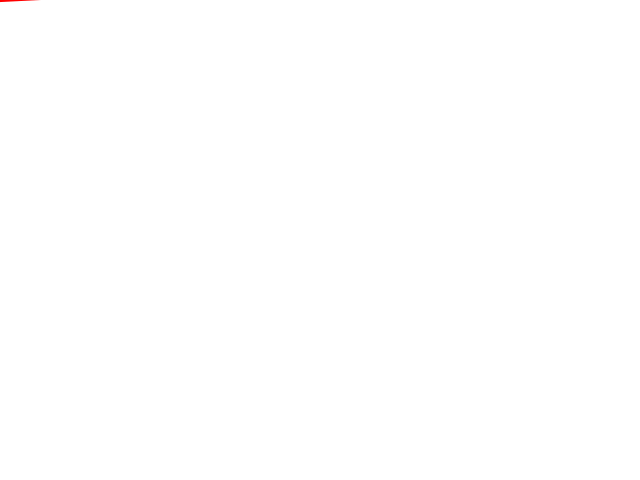
\includegraphics[scale=.4]{pants.png}
\end{center}
\caption{On the left the pair of pants $\HH/\GG$,
	on the right  the pair of pants $\HH/\GG^*$,
and in the middle the surface $\HH/(\GG\cap \GG^*)$.}
\label{fig: pants}
\end{figure}

\thebibliography{99}

\bibitem{aigner}
M. Aigner
\textit{Markov's Theorem and 100 Years of the Uniqueness Conjecture}, Springer( 2013)

\bibitem{barag}
A. Baragar,
\textit{On the Unicity Conjecture for Markoff Numbers}
Canadian Mathematical Bulletin , Volume 39 , Issue 1 , 01 March 1996 , pp. 3 - 9

\bibitem{button}
J. O. Button, 
\textit{The uniqueness of the prime Markoff numbers},
 J. London Math. Soc.
(2) 58 (1998), 9–17.

% \bibitem{cana}
% Ilke Canakci, Ralf Schiffler
% \textit{Snake graphs and continued fractions}
% European Journal of Combinatorics
% Volume 86, May 2020, 103081


\bibitem{ford}
Lester R Ford,
\textit{Automorphic Functions}

\bibitem{yi thesis}
Yi Huang
\textit{Moduli Spaces of Surfaces}e University of Melbourne Doctoral Thesis 2014
\url{https://www.yihuang.site/pdfs/yi%20huang_moduli%20spaces%20of%20surfaces%20(phd%20thesis).pdf}

\bibitem{thesis}
G. McShane, V. Sergesciu
\textit{Geometry of fermat’s sum of squares}, 2021 
\url{https://macbuse.github.io/squares.pdf}

\bibitem{thesis}
G. McShane,
\textit{Simple geodesics and a series constant over Teichmuller space}
Invent. Math. (1998)

\bibitem{mcp}
Greg McShane, Hugo Parlier,
Multiplicities of simple closed geodesics and hypersurfaces in Teichmüller space,
Geom. Topol.
Volume 12, Number 4 (2008), 1883-1919.

\bibitem{mong}
M.L. Lang, S.P Tan,
\textit{A simple proof of the Markoff conjecture for prime powers}
Geometriae Dedicata volume 129, pages15–22 (2007)

\bibitem{bob}
R. C. Penner, 
\textit{The decorated Teichmueller space of punctured surfaces}, 
Communications in Mathematical Physics 113 (1987), 299–339.

\bibitem{schmutz}
 Paul Schmutz Schaller. Geometry of Riemann surfaces based on closed geodesics. Bull. Amer.
Math. Soc. (N.S.),  1998.

\bibitem{serre}
J-P. Serre,
\textit{A Course in Arithmetic},
Graduate Texts in Mathematics,
Springer-Verlag New York
1973

\bibitem{spring}
Boris Springborn, 
\textit{The hyperbolic geometry of Markov’s theorem on Diophantine
approximation and quadratic forms.} Enseign. Math. 63 (2017)

\bibitem{saw}
Scott Wolpert,
\textit{On the Kahler form of the moduli space of once-punctured tori}, 
Comment. Math. Helv. 58(1983)246-256

\bibitem{zagier}
D. Zagier,
 \textit{A one-sentence proof that every prime p = 1 (mod 4) is a sum of two squares}, 
 American Mathematical Monthly, 97 (2): 144
 
 \bibitem{zhang}
 Y. Zhang,
 \textit{ An elementary proof of uniqueness of Markoff numbers}
 preprint, arXiv:math.NT/0606283
 
  \bibitem{zhang2}
   Y. Zhang,
 \textit{Congruence and uniqueness of certain Markoff numbers}
 Acta Arithmetica, Volume: 128, Issue: 3, page 295-301



%

%\bibitem{mcr}
%Greg McShane, Igor Rivin
%\textit{A norm on homology of surfaces and counting simple geodesics}
%International Mathematics Research Notices, Volume 1995, Issue 2, 1995
%
%
%
%\bibitem{ra}
%M. Rabideaua, R. Schiffler,
%\textit{Continued fractions and orderings on the Markov numbers},
%Advances in Mathematics Vol 370,  2020.
%
%
%
%\bibitem{vu}
%C Lagisquet and E. Pelantová and S. Tavenas and L. Vuillon,
%\textit{On the Markov numbers: fixed numerator, denominator, and sum conjectures.}
%\url{https://arxiv.org/abs/2010.10335}
%


%\bibitem{Gui}
%L. Guillop\'e, Laurent(F-GREN-F)
%Sur la distribution des longueurs des g\'eod\'esiques ferm\'ees d'une surface compacte \`a bord totalement g\'eod\'esique. 
%Duke Math. J. 53 (1986), no. 3, 827-848. 

%\bibitem{MC}
%C. L. Mallows and J. M. C. Clark. 
%{\it Linear-intercept distributions do not characterize plane sets}
% Journal of Applied Probability, 7(1):240-244, 1970.
% 
% \bibitem{Masai-McShane}
% Masai, Hidetoshi and Greg McShane,
% ``On systoles and ortho spectrum rigidity'', preprint.
% \bibitem{MMc}
% Masai, Hidetoshi, and Greg McShane. "Equidecomposability, volume formulae and ortho spectra." Algebraic \& Geometric Topology 13.6 (2013): 3135-3152.
 



\end{document}

